% Template:     Auxiliar LaTeX
% Documento:    Archivo principal
% Versión:      8.3.3 (20/01/2025)
% Codificación: UTF-8
%
% Autor: Pablo Pizarro R.
%        pablo@ppizarror.com
%
% Manual template: [https://latex.ppizarror.com/auxiliares]
% Licencia MIT:    [https://opensource.org/licenses/MIT]

% CREACIÓN DEL DOCUMENTO
\documentclass[
	spanish, % Idioma: spanish, english, etc.
	letterpaper, oneside
]{article}

% INFORMACIÓN DEL DOCUMENTO
\def\documenttitle {Auxiliar 5}
\def\documentsubject {Dinámica}

\def\documentauthor {Nombre del autor}
\def\coursename {Mecánica}
\def\coursecode {FI-2001}

\def\universityname {Universidad de Chile}
\def\universityfaculty {Facultad de Ciencias Físicas y Matemáticas}
\def\universitydepartment {Departamento de la Física}
\def\universitydepartmentimage {departamentos/fcfm}
\def\universitydepartmentimagecfg {height=1.75cm}
\def\universitylocation {Santiago de Chile}

% EQUIPO DOCENTE
\def\teachingstaff {
	\textbf{Profesor: Claudia Scóccola} \\
	Auxiliares: Jorge Barja, Clemente Miranda, Matías Zúñiga \\
	Ayudante: Mario Calderón  \\
}

% IMPORTACIÓN DEL TEMPLATE
\input{template}

% INICIO DE PÁGINAS
\begin{document}

% CONFIGURACIÓN DE PÁGINA Y ENCABEZADOS
\templatePagecfg

% ======================= INICIO DEL DOCUMENTO =======================

% \newboxquestion{P1}\\

% Considere una bolita de masa $m$ ensartada en una barra de manera que puede deslizar sin roce por ella. La masa está atada mediante un resorte, de constante elástica $k$ y largo natural $l_0$, a un extremo de la barra, y esta última, a su vez, gira c/r al mismo extremo en un plano horizontal con velocidad angular $w$ constante. En $t=0$ la bolita se suelta con resorte comprimido en $l_0/2$ y $\dot{\rho}(0) = 0$:

% \begin{enumerate}[label=\alph*)]
%     \item ¿Qué relación deben cumplir $m,k$ y $w$ para que la bolita realice un movimiento armónico simple a lo largo de la barra?.
%     \item Determine la compresión del resorte como función del tiempo..

% \end{enumerate}


% \begin{figure}[ht] % [h] indica que se coloca la imagen aquí (here)
%     \centering % Centra la imagen
%     
\includegraphics[width=0.4\textwidth]{p1.png} % Ajusta el tamaño de la imagen
%     \caption{Pregunta 1.} % Subtítulo de la imagen
%     \label{fig:p1} % Etiqueta opcional para referencias
% \end{figure}

\newboxquestion{P1}\\

Una partícula de masa $m$ desliza por una pared vertical empujada por un resorte de constante elástica
$k$. El otro extremo está fijo en el punto $O$, tal como lo muestra la figura. La distancia entre $O$ y la pared
es $b$ (distancia $OA$) y el largo natural del resorte es $l_0 = 2b$. Entre la partícula y la pared existe un roce
caracterizado por el coeficiente $\mu$ (cinético y estático).

\begin{enumerate}[label=\alph*)]

    \item  ¿Qué condición debe cumplir $\mu$ tal que al dejar la partícula en reposo en el punto $A$, ésta comience a descender?

    \item Si $\mu$ cumple la condición de $(a)$ y la partícula es liberada desde el reposo en el punto $A$, determine la magnitud de la normal que la pared ejerce sobre la partícula en función del ángulo $\alpha$. Indique el ángulo $\alpha$ en que la partícula se separa de la pared.

\end{enumerate}

\begin{figure}[ht] % [h] indica que se coloca la imagen aquí (here)
    \centering % Centra la imagen
    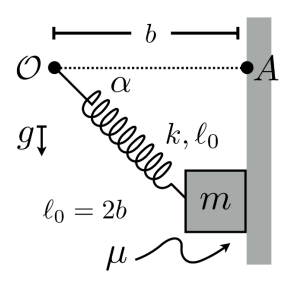
\includegraphics[width=0.3\textwidth]{P1.png} % Ajusta el tamaño de la imagen
    \caption{Pregunta 1.} % Subtítulo de la imagen
    \label{fig:p1} % Etiqueta opcional para referencias
\end{figure}

% \begin{figure}[h]
%     \centering
%     \begin{subfigure}{0.48\textwidth}
%         \centering
%         
\includegraphics[width= 0.6\textwidth]{p1.png}
%         \caption{Pregunta 1}
%         \label{fig:p3}
%     \end{subfigure}
%     \hfill
%     \begin{subfigure}{0.48\textwidth}
%         \centering
%         
\includegraphics[width= 0.8\textwidth]{p3.png}
%         \caption{Pregunta 2}
%         \label{fig:p4}
%     \end{subfigure}
%     \label{fig:preguntas1}
% \end{figure}

\newpage

\newboxquestion{P2} \\


Considere un sistema compuesto por un resorte y una masa que se encuentran al borde de una piscina muy profunda como se indica en la figura. El resorte es de largo natural $l_0$ y constante elástica $k$. A éste se fija una pared móvil de masa despreciable. El sistema se prepara de modo que la partícula puntual de masa $m$ se coloca junto a esta pared en su posición de compresión máxima, es decir en $x = −l_0$, según el sistema de coordenadas que se muestra en la figura, y se suelta desde el reposo. Se pide:

\begin{enumerate}[label=\alph*)]
    \item ¿Cuál es la condición que asegura que la masa $m$ se moverá desde $x = −l_0$?
    \item Encuentre el valor máximo de $\mu_d$ que permita a la masa llegar al borde de la piscina ($x = 0$) con velocidad no nula. Entregue el valor de ésta velocidad no nula.
    \item Considere que la masa entra a la piscina inmediatamente cuando $x > 0$. Una vez que entra, la masa experimenta una fuerza de roce viscoso lineal, de constante $\gamma$. Suponga además que no hay fuerza de empuje (la masa es puntual). Determine entonces el alcance máximo que alcanzará la masa y su velocidad límite.
\end{enumerate}

\begin{figure}[ht] % [h] indica que se coloca la imagen aquí (here)
    \centering % Centra la imagen
    
\includegraphics[width=0.4\textwidth]{P2.png} % Ajusta el tamaño de la imagen
    \caption{Pregunta 2.} % Subtítulo de la imagen
    \label{fig:p2} % Etiqueta opcional para referencias
\end{figure}


% \newboxquestion{P3}\\


% Una partícula $P$ de masa $m$ puede moverse sin roce por el interior de un tubo horizontal de largo $2R$. El tubo gira en torno a su punto medio con velocidad angular constante $w_0$. La partícula está unida al extremo de un resorte de constante $k = 2mw_0$ y largo natural $l_0 > R$ cuyo extremo está unido al tubo en el punto $A$, como se muestra en la figura. Inicialmente $P$ está en reposo, ubicada en el punto medio del tubo.

% \begin{enumerate}[label=\alph*)]
%     \item Determine la distancia de la partícula al centro del tubo en todo instante de tiempo.
  
%     \item  Si $l_0 = \alpha R$ encuentre el valor $\alpha _{max}$ que asegura que $P$ nunca choca con el punto $B$ del tubo
  
%     \item Encuentre la reacción que ejerce el tubo a la partícula, sus valores máximos y mínimos, además de los instantes en que esto ocurre.\\
%     Hint: Durante el movimiento, la partícula nunca cruza el punto medio del tubo

% \end{enumerate}

% % \begin{figure}[ht] % [h] indica que se coloca la imagen aquí (here)
% %     \centering % Centra la imagen
% %     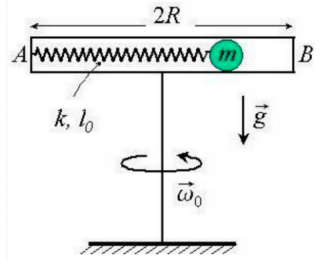
\includegraphics[width=0.3\textwidth]{P3.png} % Ajusta el tamaño de la imagen
% %     \caption{Pregunta 3.} % Subtítulo de la imagen
% %     \label{fig:p2} % Etiqueta opcional para referencias
% % \end{figure}

% \begin{figure}[h]
%     \centering
%     \begin{subfigure}{0.48\textwidth}
%         \centering
%         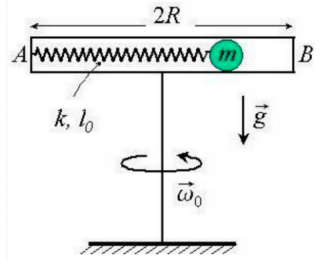
\includegraphics[width= 0.7\textwidth]{P3.png}
%         \caption{Pregunta 3}
%         \label{fig:p3}
%     \end{subfigure}
%     \hfill
%     \begin{subfigure}{0.48\textwidth}
%         \centering
%         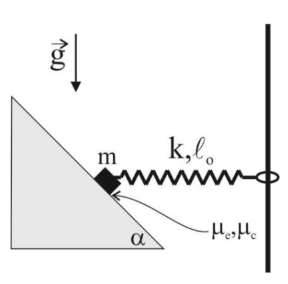
\includegraphics[width= 0.7\textwidth]{P4.png}
%         \caption{Pregunta 4}
%         \label{fig:p4}
%     \end{subfigure}
%     \label{fig:preguntas1}
% \end{figure}


\newboxquestion{P3} \textbf{(Propuesto)}\\

Considere el siguiente modelo simplificado de la generación de un terremoto por convergencia de placas. La
partícula de masa $m$ se encuentra apoyada sobre una cuña de ángulo $\alpha$ respecto de la horizontal, a la vez que
ligada a una barra fija vertical mediante un resorte horizontal de constante elástica $k$ y largo natural $\ell_0$. Entre
la partícula y la cuña existen coeficientes de roce estático y cinético de coeficientes $\mu _e$ y $\mu _c$, respectivamente.

\begin{enumerate}[label=\alph*)]
    \item Si la cuña se acerca muy lentamente a la barra vertical, determine el largo del resorte en el momento que se vence el roce estático y la partícula asciende pendiente arriba sobre la cuña (es decir, el momento en que ocurre el terremoto).
    \item Determine el desplazamiento total de la partícula hasta que se detiene nuevamente. Suponga que en este proceso la cuña se mantiene en reposo, el resorte se mantiene horizontal (su otro extremo asciende por la barra vertical), y la partícula no se separa de la cuña.
\end{enumerate}

\begin{figure}[ht] % [h] indica que se coloca la imagen aquí (here)
    \centering % Centra la imagen
    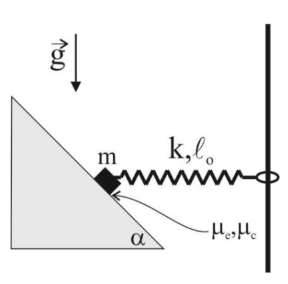
\includegraphics[width=0.3\textwidth]{P4.png} % Ajusta el tamaño de la imagen
    \caption{Pregunta 3.} % Subtítulo de la imagen
    \label{fig:p3} % Etiqueta opcional para referencias
\end{figure}

% FIN DEL DOCUMENTO
\end{document}